\chapter{Design and Framework}


\section{System Design}

\begin{sidewaysfigure}
    \centerline{
    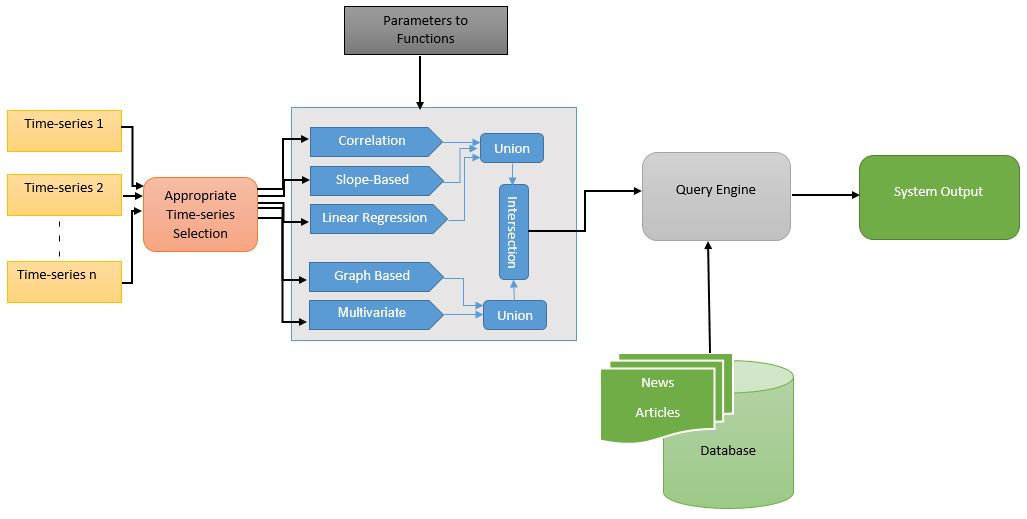
\includegraphics[width=0.9\textwidth]{System_updated.JPG}
    }
    \caption{System Framework}
    \label{fig:SystemDesign}
\end{sidewaysfigure}

Figure \ref{fig:SystemDesign} explains the overall design of the system and its modules.\\
\\
We have multiple time-series as input. These time-series are to be read from file manually using python script and generate 2D list of the time-series. These 2D lists has first column as date and then we have one or more columns corresponding to one or more values for that date. In the next stage depending upon what time-series we need to compare, we select appropriate time-series and pass this as input to various functions. Note that it is required to have all time-series of equal length and time period for which time-series are considered should be same for all time-series.\\
\\
We have implemented 5 functions till now as shown in figure \ref{fig:SystemDesign} viz. Correlation, Slope Based, Linear Regression, Graph Based and Multivariate. Detail about each function is explained in the next section. These functions takes either 2 or multiple time-series as input and has various parameters. Depending upon how time-series should behave with respect to each other (directly propotional or inversaly propotional) parameteres are tuned. We take union of results of first three functions and rest of the two functions as shown in figure. After taking union, we take intersection of two results of union as shown in figure. This is final result produced by the system. This result states the anomalies in the time-series.\\
\\
To verify result produced by system, we match it with the news articles present for the test case considered (here onion test case). We match system results with news articles present and check how well system is performing. Note that it is not necessary that for each and every anomaly case, we have news article present. If not, then we manually check behavior of time-series on that date. If some news articles do not match with system result then we also study, why they did not match and what are limitations of system.\\


\section{Test Criterion for Hypothesis}

In the last chapter, we stated some hypothesis. Now, here we state what tests can be performed to detect anomalies for each of the hypothesis.

\subsection{Hypothesis 1}

In this, we use three functions:

\begin{itemize}

\item Starting with granularity of year-wise, find out cross-correlation, considering various lag factor up to 15,  between arrival and wholesale and check that overall it is positive or negative.

\item Go on decrease the granularity. Next will be season-wise. For a particular season, how arrival and wholesale price are behaving. Point out where, this correlation becomes positive.

\item Similar thing can be done for month-wise as well as fortnight data.

\item Note that, correlation mentioned here is just one of the method. There can be various other methods to define the behavior of 2 time-series.

\item \textbf{Slope Based Detection:} Calculate the slope of both time-series daywise and compare. \textit{Assumption:} Data is smoothed. Since day-wise is taken, if data is not smoothed then it may generate many “spikes”. So if data is not smoothed, then before applying this technique, either apply smoothing or take weekly average. If granularity of data is daywise, then smoothing can help. If data is reported once-twice weekly, then taking average weekly and then calculating slope day-wise may help.

\item \textbf{Linear Regression Based Method:} We can train model using linear regression. Then find out the difference between actual and predicted value for each of the data point and plot a histogram. From these points we can try to find out points which are going very much out of the way using method like MAD test.

\end{itemize}

\subsection{Hypothesis 2}

\begin{itemize}

\item Starting with granularity of year-wise, find out cross-correlation, considering various lag factor up to 15,  between arrival and wholesale and check that overall it is positive or negative.

\item Go on decrease the granularity. Next will be season-wise. For a particular season, how arrival and wholesale price are behaving. Point out where, this correlation becomes positive.

\item Similar thing can be done for month-wise as well as fortnight data.

\item Note that, correlation mentioned here is just one of the method. There can be various other methods to define the behavior of 2 time-series.

\item \textbf{Slope Based Detection:} Calculate the slope of both time-series daywise and compare. \textit{Assumption:} Data is smoothed. Since day-wise is taken, if data is not smoothed then it may generate many “spikes”. So if data is not smoothed, then before applying this technique, either apply smoothing or take weekly average. If granularity of data is daywise, then smoothing can help. If data is reported once-twice weekly, then taking average weekly and then calculating slope day-wise may help.

\item \textbf{Linear Regression Based Method:} We can train model using linear regression. Then find out the difference between actual and predicted value for each of the data point and plot a histogram. From these points we can try to find out points which are going very much out of the way using method like MAD test.

\item Spike Detection methods

\end{itemize}

\subsection{Hypothesis 3}

\begin{itemize}

\item One can use prediction based model like ARIMA \cite{arima} to test this hypothesis. If method mentioned in \cite{arima} is used then there is no need to align time-series into phase, as method mentioned in it take care of it. One can train the model considering some period for 8 years and can be tested on remaining 2 years. Difference in actual and predicted value is seen and one above some threshold value is reported. Also, while generating model, different window size can be considered. If some other technique is used, then one may need to align time series into common phase. That can be done using cross-correlation method, considering lag factor of around 15 days. Lag with the highest correlation value is considered.

\item One can also apply graph based anomaly detection technique as mentioned in \cite{nasa} to find out malicious behavior.

\end{itemize}

\subsection{Hypothesis 4}


Here, we need to combine data of multiple places into one, to find out the combined behavior and then compare it with each of the mandi. One of the technique, to combine multiple series is,

\begin{itemize}

\item For Arrivals: take sum from all Mandis
\item For Wholesale-price: Take average
\item Apart from center, if one wants to combine statewise, then for retail price also, one can take average for retail price

\end{itemize}

Other technique, to combine multiple time series is, subspace based transformation, as mentioned in \cite{phdthesisdc}. Then, to compare behavior of each particular mandi time-series with the aggregated one, techniques mentioned to test hypothesis 1 or 2 can be used.

\textbf{Note (Applicable to Onion Case):} Results returned by H1 and H2, consists of all the time periods where arrival-wholesale price and wholesale price-retail price pairs go out of line. There may be case where, for each time of that year it may be going out of line and might not be anomaly. So, to remove such false positives, we can take intersection of results of H1 and results of H3. Similar thing can be done with H2 also, by taking  intersection of results of H2 and results of H3.


